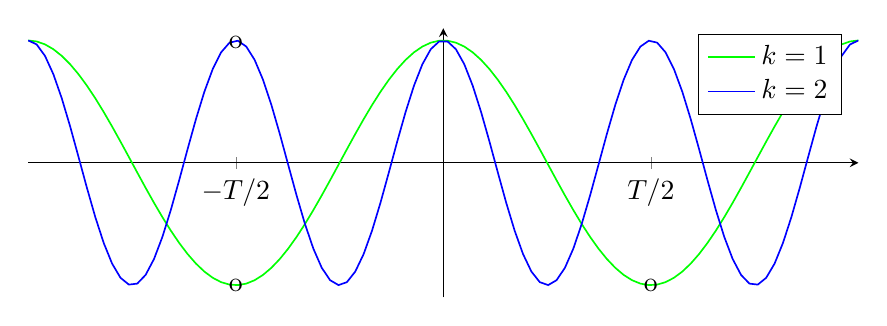
\begin{tikzpicture}
    \begin{axis}[
        width = \linewidth,
        height = 5cm,
        axis x line=center,
        axis y line=middle,
        samples=100,
        ymin=-1.1, ymax=1.1,
        xmin=-pi, xmax=pi,
        ytick=\empty,
        xtick={-pi/2,pi/2},
        xticklabels={$-T/2$,$T/2$}
        ]
        \addplot [semithick, green, domain=-pi:pi] {cos(2*deg(x))};
        \addlegendentry{$k=1$};
        \addplot [semithick, blue, domain=-pi:pi] {cos(4*deg(x))};
        \addlegendentry{$k=2$};
        \draw (axis cs: -1.57,0.98) node {o};
        \draw (axis cs: -1.57,-1) node {o};
        \draw (axis cs:  1.57,-1) node {o};
    \end{axis}
\end{tikzpicture}
